\documentclass{article}

\usepackage[version=3]{mhchem} % Package for chemical equation typesetting
\usepackage{siunitx} % Provides the \SI{}{} and \si{} command for typesetting SI units
\usepackage{natbib} % Required to change bibliography style to APA
\usepackage{graphicx}
\usepackage{mathtools}
\usepackage{amssymb}
\usepackage{amsthm}
\usepackage[italian]{babel}
\usepackage{stackengine}
\usepackage{graphicx,ifthen}
\usepackage{amsmath}
\usepackage{hyperref}
\usepackage{upgreek}
\usepackage{bm}

\renewcommand{\labelenumi}{\alph{enumi}.} % Make numbering in the enumerate environment by letter rather than number (e.g. section 6)

\title{Esperienza IV: \\ polarimetro di Laurent}
\author{Manuel G. Moretti\footnote{email: manuel.moretti560@edu.unito.it}}
\date{Luglio 2024}

\begin{document}

\maketitle

\begin{center}
\begin{tabular}{l r}
Esperimentazioni II corso B & A.A. 2023/24 \\
Modulo II & Universit\'{a} degli Studi di Torino \\
\end{tabular}
\end{center}

\begin{abstract}
In questa esperienza si è determinata la concentrazione di fruttosio e saccarosio in soluzione acquosa tramite un polarimetro di Laurent. Si è inoltre verificata la legge di Malus facendo uso di un laser passante attraverso un filtro polarizzatore.
\end{abstract}

\section{Obiettivi della misura}
Gli obiettivi di questa esperienza sono i seguenti: determinare la concentrazione di fruttosio e saccarosio in soluzione acquosa, tramite l'utilizzo di un polarimetro di Laurent e avvalendoci della legge di Biot per il potere rotatorio specifico; verificare la legge di Malus per un laser passante attraverso un filtro polarizzatore in modo da poter analizzare la luce laser.

\section{Configurazione dell'apparato sperimentale}
L'apparato sperimentale consiste in un polarimetro di Laurent in cui possono essere posizionate delle provette contenenti la soluzione di acqua e fruttosio, o saccarosio. Il polarimetro di Laurent sfrutta una lampada al sodio come sorgente luminosa. Un primo prisma di Nicol permette il passaggio solo alla componente polarizzata in una certa direzione. Quest'ultima ruota mentre la luce attraversa la provetta da analizzare. Un secondo prisma di Nicol, corredato di goniometro con nonio, funge da analizzatore per misurare la rotazione. Inoltre, il polarimetro sfrutta una lamina a mezz'onda in modo da rendere più precisa l'individuazione del punto di uguale illuminazione in condizione di minima intensità.
\begin{figure}[ht]
    \centering
    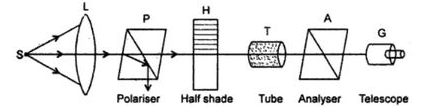
\includegraphics[width=0.6\linewidth]{Immagini/schema polarimetro.png}
    \caption{diagramma del polarimetro di Laurent}
    \label{fig:schema polarimetro}
\end{figure}
Chiaramente, l'esperimento viene condotto usando fruttosio e saccarosio in quanto queste sono molecole otticamente attive, rispettivamente aventi potere rotatorio specifico $\alpha$ di -92.00 dm$^{-1}$cm$^3$g$^{-1}$ e 66.37 dm$^{-1}$cm$^3$g$^{-1}$.

Per la seconda parte dell'esperienza l'apparato sperimentale consiste in un laser, un filtro polarizzatore e in una fotocellula collegata ad un microamperometro. Il filtro analizzatore può essere ruotato di 360° in modo da poter cambiare l'inclinazione dell'asse ottico del filtro.

\section{Raccolta ed elaborazione dei dati}
\subsection{Stima delle concentrazioni tramite polarimetro di Laurent}
La raccolta dati è consistita nel preparare quattro provette contenti rispettivamente 0.5, 1, 1.5 e 2 grammi di fruttosio in soluzione acquosa, e altrettante contenti invece saccarosio sempre nelle stesse concentrazioni. Si è quindi proceduto con il posizionare una alla volta le provette all'interno del polarimetro. Quindi, per ognuna di queste si è cercato l'angolo al quale avveniva la condizione di uguale illuminazione in minima intensità. Per ogni provetta si sono effettuate quattro misure. Inoltre, questo processo deve essere effettuato anche con il polarimetro vuoto in modo da poter determinare l'angolo di rotazione $\alpha$ del piano di polarizzazione come
\begin{equation}
    \label{eq:angolo alpha}
    \alpha=\theta-\theta ',
\end{equation}
dove $\theta$ indica la misura effettuata senza provetta, mentre $\theta '$ con quest'ultima. I dati ottenuti in questa parte di esperienza sono raccolti nella seguente tabella.
\begin{table}[h]
    \centering
    \begin{tabular}{|c|c|c|}
        \hline
        \textbf{Quantità di soluto [g]} & \bm{$\alpha$}\textbf{ fruttosio [deg]} & \bm{$\alpha$} \textbf{saccarosio [deg]} \\
        \hline
        $0.5 \pm 0.1$ & $-4.82 \pm 0.27$ & $6.04 \pm 0.05$ \\
        \hline
        $1.0 \pm 0.1$ & $-8.87 \pm 0.77$ & $7.53 \pm 0.10$ \\
        \hline
        $1.5 \pm 0.1$ & $-14.39 \pm 0.68$ & $9.11 \pm 0.09$ \\
        \hline
        $2.0 \pm 0.1$ & $-19.96 \pm 0.59$ & $12.21 \pm 0.19$ \\
        \hline
    \end{tabular}
    \caption{Quantità di soluto e valori di $\alpha$ per fruttosio e saccarosio}
    \label{tab:angoli zuccheri}
\end{table}

Ora facendo uso della legge di Biot per il potere rotatorio specifico è possibile determinare la concentrazione $c$ di sostanza nelle rispettive soluzioni
\begin{equation}
    \label{eq:legge di biot}
    \alpha=kcl\quad\therefore\quad c=\frac{\alpha}{kl},
\end{equation}
dove $l$ indica la lunghezza della provetta che vale $l=(20.0\pm0.1)$ cm e $k$ indica il potere rotatorio specifico delle sostanza prima citati.
\subsection{Verifica della legge di Malus}
La raccolta dei dati è consistita in una serie di misure della corrente generata dalla luce laser impattante la fotocellula in seguito al passaggio attraverso il filtro polarizzatore. Il filtro, partendo dalla posizione iniziale corrispondente all'angolo 0° sulla scala graduata, è stato fatto ruotare di 360° con un passo di 10° ogni misura, ottenendo pertanto trentasei misure dell'intensità $I$ della luce laser. 

La legge di Malus mette in relazione l'intensità iniziale $I_0$ del raggio laser con l'intensità $I$ del raggio in seguito al passaggio attraverso il filtro tramite l'equazione
\begin{equation}
    \label{eq:legge di malus}
    I=I_0\cos^2{\theta},
\end{equation}
dove $\theta$ è l'angolo dell'asse ottico del filtro.

\section{Risultati e conclusioni}
I risultati raccolti nella tabella \ref{tab:angoli zuccheri} possono essere sostituiti nell'equazione \eqref{eq:legge di biot}, insieme ai valori di $\alpha$ e $l$, così da ottenere le seguenti stime della concentrazioni delle due sostanze in soluzioni.
\begin{table}[h]
    \centering
    \begin{tabular}{|c|c|c|}
        \hline
        \textbf{Quantità di soluto [g]} & \textbf{$c$ fruttosio [g/cm$^3$]} & \textbf{$c$ saccarosio [g/cm$^3$]} \\
        \hline
        $0.5 \pm 0.1$ & $0.026\pm0.002$ & $0.046\pm0.001$ \\
        \hline
        $1.0 \pm 0.1$ & $0.048\pm0.004$ & $0.057\pm0.001$ \\
        \hline
        $1.5 \pm 0.1$ & $0.078\pm0.004$ & $0.069\pm0.001$ \\
        \hline
        $2.0 \pm 0.1$ & $0.108\pm0.003$ & $0.092\pm0.002$ \\
        \hline
    \end{tabular}
    \caption{Stime concentrazioni di fruttosio e saccarosio}
    \label{tab:concentrazioni zuccheri}
\end{table}

I valori di $c$ ottenuti nella tabella \ref{tab:concentrazioni zuccheri} devono essere confrontati con i valori di concentrazioni ricavabili nota la composizione della soluzione di acqua e fruttosio, o saccarosio. I valori di $c$ calcolati in questo modo sono raccolti nella seguente tabella.
\begin{table}[h]
    \centering
    \begin{tabular}{|c|c|c|}
        \hline
        \textbf{Quantità di soluto [g]} & \textbf{$c$ fruttosio [g/cm$^3$]} & \textbf{$c$ saccarosio [g/cm$^3$]} \\
        \hline
        $0.5 \pm 0.1$ & $0.024\pm0.005$ & $0.025\pm0.005$ \\
        \hline
        $1.0 \pm 0.1$ & $0.048\pm0.005$ & $0.048\pm0.005$ \\
        \hline
        $1.5 \pm 0.1$ & $0.074\pm0.005$ & $0.072\pm0.005$ \\
        \hline
        $2.0 \pm 0.1$ & $0.095\pm0.005$ & $0.098\pm0.005$ \\
        \hline
    \end{tabular}
    \caption{Stime concentrazioni di fruttosio e saccarosio note le soluzioni}
    \label{tab:concentrazioni zuccheri note soluzioni}
\end{table}

Effettuando quindi un test di Gauss tra le misure di $c$ per le rispettive sostanza e concentrazioni si trova che i valori di $c$ nelle tabelle \ref{tab:concentrazioni zuccheri}  e \ref{tab:concentrazioni zuccheri note soluzioni} riferiti alle soluzioni di fruttosio per le grammature di 0.5, 1 e 1,5 e alle soluzioni di saccarosio per le grammature di 1, 1.5 e 2, sono compatibili tra loro ad un livello si significatività del 5\%. Discorso diverso deve essere fatto per le provette di fruttosio e saccarosio rispettivamente per le grammature di 2 e 0.5. Queste due coppie di stime di $c$ non risultano infatti compatibili ad un livello si significatività del 5\%. Questo fatto può essere spiegato da una probabile contaminazione delle provette che, essendo state usate svariate volte in esperimenti precedenti,  potrebbero contenere alcuni residui di soluto. Inoltre, i cucchiai usati per raccogliere i due zuccheri sono stati scambiati accidentalmente negli esperimenti precedenti a questo. Questi due fattori potrebbero essere stati la causa di questa incompatibilità tra le misure effettuate con il polarimetro e i valori calcolati nota la composizione della soluzione

I dati raccolti nella seconda parte dell'esperienza invece possono essere rappresentati in un grafico mostrante l'andamento dell'intensità dell'onda al variare dell'angolazione del filtro polarizzatore.
\begin{figure}[h]
    \centering
    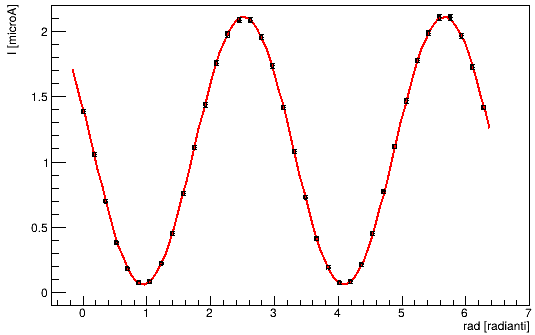
\includegraphics[width=0.7\linewidth]{Immagini/andamento I.png}
    \caption{grafico di $I(\theta)$}
    \label{fig:andamento I}
\end{figure}

Effettuando dunque una regressione sui dati in figura \ref{fig:andamento I} con la legge di Malus, enunciata nell'equazione \eqref{eq:legge di malus}, ovvero con una funzione del tipo $f(x)=A\cos^2{x}$, si trova che il modello si adatta a tutto il range di dati verificando dunque la legge di Malus.

\end{document}